\chap{Activities in Obergurgl}
\paragraph{Downhill skiing}
There are several shops in Obergurgl where you can buy or rent skiing equipment. The one closest to the skiing lifts is Scheiber Sport (https://www.scheibersport.com/). Skiing passes can be bought right next to the skiing lifts. If you are new to skiing, you can book lessons at one of the skiing schools in Obergurgl (http://www.alpinsport-obergurgl.at or www.skischule-obergurgl.com). 

\paragraph{Skating}
There is an ice-skating rink in Obergurgl, which is opened daily from 3:30 pm to 10:30 pm. Ice-skates can be rented at the place. We are planning to organize a friendly game of ice-hockey during the winterschool, so if you are interested contact Janko from the organizing team. 

\paragraph{Sledding}
In Hochgurgl a three kilometer long natural toboggan run leads from the top station of Hochgurglbahn mountain gondola down to the valley. Toboggans can be rented at the base station of the Hochgurglbahn mountain gondola and at Scheiber Sport at Top Hotel in Hochgurgl for 7 euro. Lift tickets can be bought for 6 euro per ride, or for 20 euro for a full day. 

\paragraph{Cross Country Skiing}  Obergurgl-Hochgurgl boasts perfectly groomed tracks for Nordic sport fans, with 12 kilometers of Nordic ski trails, 3 kilometers of practicing tracks and 1 kilometer equipped with floodlights in Hochgurgl. Information about the tracks can be found at the website (https://www.obergurgl.com/cross-country-skiing), tourist information or ski shops. 

\paragraph{Winter hiking} Explore the most beautiful spots on 12 km of cleared winter hiking trails leading right across snow-covered forests, white fields or along mountain brooks. Quaint mountain huts invite you to enjoy a well-deserved snack. 
In addition, the snowshoeing terrain is almost unlimited. You can either take part in one of the scenic guided snowshoe hikes or explore the winter wonderland on your own. Snow shoes can be rented at the ski schools 

\paragraph{Public transport} There are busses towards Hochgurgl, stopping at the Festkogelbahn and Hochgurglbahn, leaving from Obergurgl Zentrum every 10 minutes in the morning and afternoon. The same applies for the opposite direction. A single ticket costs 2,90. 

\begin{figure}
	\centering
	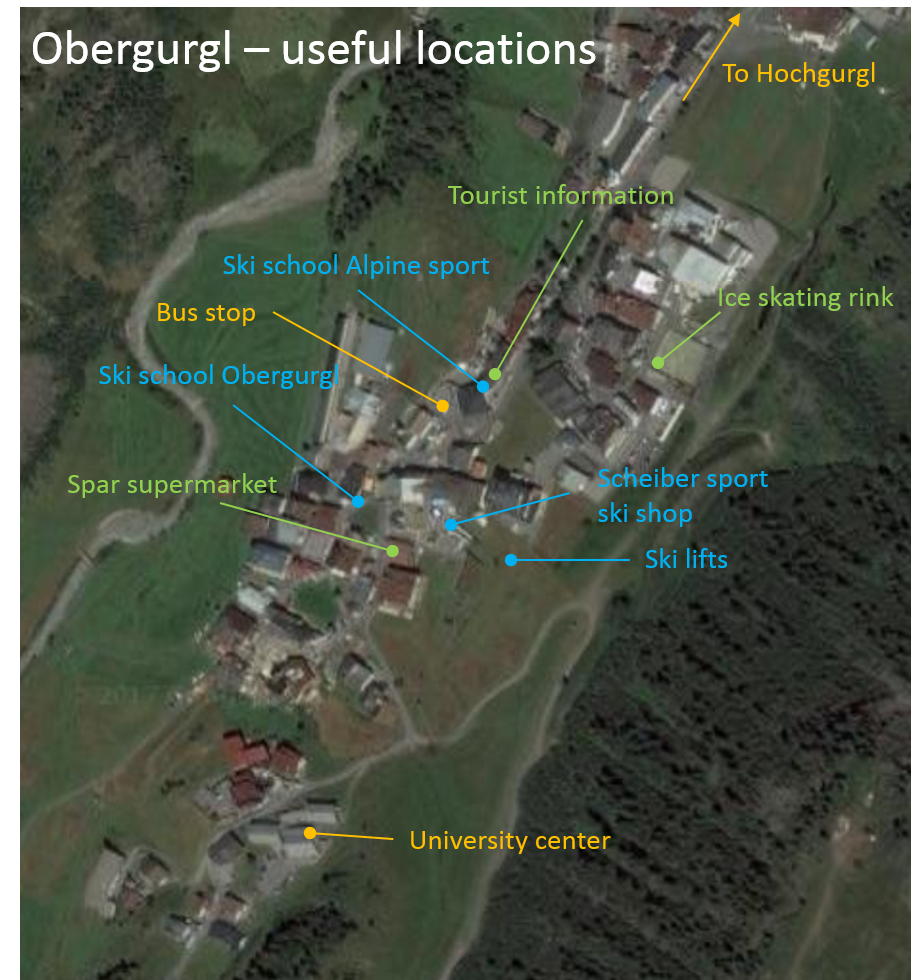
\includegraphics[width=1\textwidth]{map}

\end{figure}


